\section{Experimental Evaluation}
\label{sec:results}

We evaluate \Treebeard{} on four different target processors, an NVIDIA RTX 4060 GPU (8GB RAM, CUDA 11.8),
an NVIDIA T400 GPU (2GB RAM, CUDA 11.5), an AMD MI210 GPU (64GB RAM, ROCm 6.0.2) and an 
Intel Core i9-11900K CPU (16 virtual cores, 128 GB RAM). We compare \Treebeard{} with 
four other systems, NVIDIA RAPIDs v23.10, Tahoe, XGBoost v1.7.6 and \TreebeardOLD{} CPU. 
We measure both kernel time and total time (including data transfer to the GPU and results back) 
for RAPIDs and \Treebeard{}. Tahoe only allows us to measure the kernel time since it is written
as an executable that performs inference repeatedly on the same data that is transferred to the GPU once.

We use two sets of benchmarks to perform the comparison.
We use 8 real-world models trained on data from the Intel Machine 
Learning Benchmark suite~\cite{MLBenchmarks}. These models were also
used to evaluate \TreebeardOLD{}\cite{Treebeard}.
To enable more exhaustive evaluation we generated 700 random models with
varying number of trees (100---1000) and features (powers of two in the range 8---1024). 
Each tree has leaves at depths 2 to a maximum depth of 6, 7 or 8.
For \Treebeard{}, we use schedules found using the schedule exploration
heuristic (Section \ref{sec:exploring}) unless otherwise specified.

\subsection{Performance comparisons on NVIDIA GPUs}

\begin{figure}[htb]
  \centering
  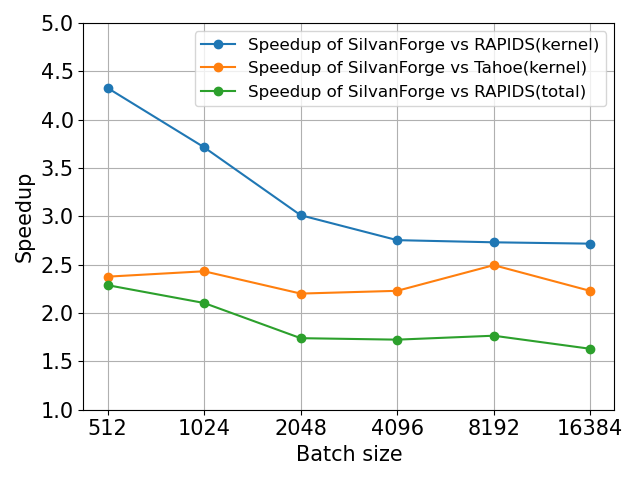
\includegraphics[width=0.75\linewidth]{figures/geomean_speedup_4060_kernel_time_total_time.png}
  \caption{\Treebeard{} vs RAPIDs and Tahoe kernel time and total time speedup (geomean over real-world 
  benchmarks) across batch sizes on NVIDIA RTX 4060}
  \label{Fig:TBvsRAPIDsTahoe_4060_Speedup}
\end{figure}

% \begin{figure}[htb]
%   \centering
%   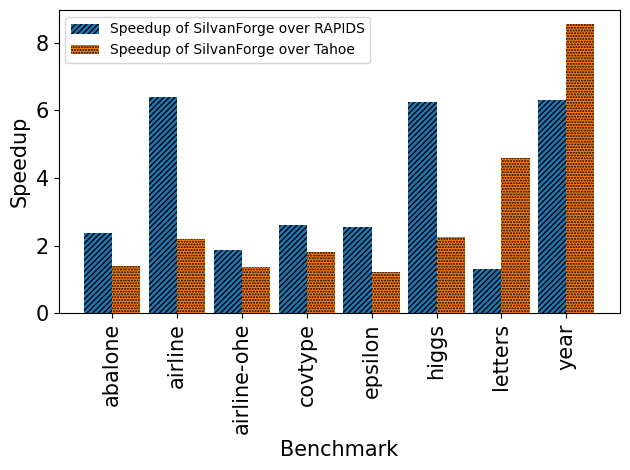
\includegraphics[width=0.75\linewidth]{figures/geomean_speedup_4060_bar_graph.png}
%   \caption{\Treebeard{} vs RAPIDs and Tahoe kernel time and total time speedup on NVIDIA RTX 4060 for individual benchmarks (geomean over all batch sizes).
%   \TODO{Add bar for total time. Add whiskers to each bar to show range of speedups.}}
%   \label{Fig:TBvsRAPIDsTahoe_4060_Speedup}
% \end{figure}

\begin{figure}[htb]
  \centering
  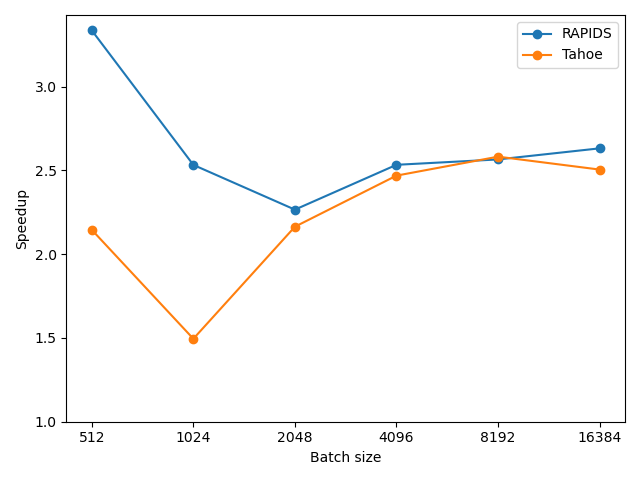
\includegraphics[width=0.75\linewidth]{figures/geomean_speedup_T400_kernel_time.png}
  \caption{\Treebeard{} vs RAPIDs and Tahoe kernel time and total time speedup (geomean over real-world 
  benchmarks) across batch sizes on NVIDIA T400.}
  \label{Fig:TBvsRAPIDsTahoe_T400_Speedup}
\end{figure}

\begin{figure*}[ht]
  \centering
  \begin{subfigure}[b]{.45\textwidth}
    \subcaptionbox*{}{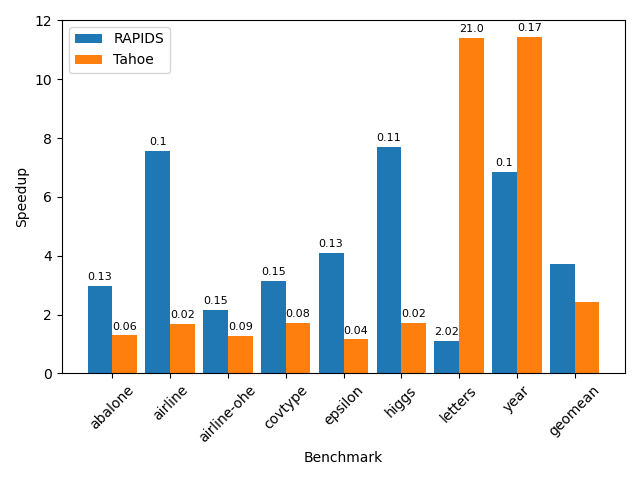
\includegraphics[width=\textwidth]{figures/speedup_bar_graph_1024.png}}
    \caption{Batch size 1024}
  \end{subfigure}
  \begin{subfigure}[b]{.45\textwidth}
    \subcaptionbox*{}{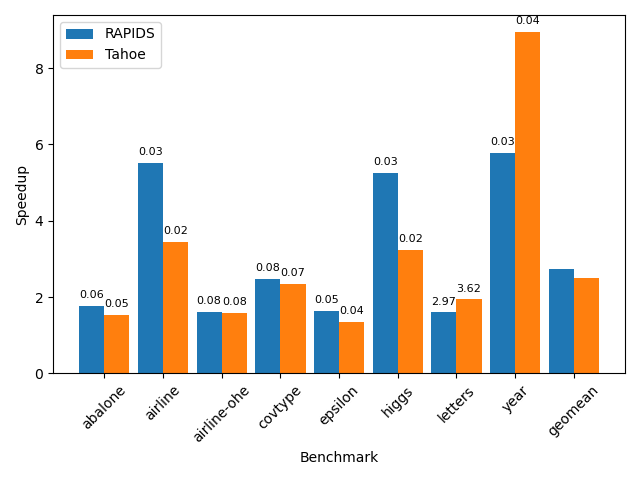
\includegraphics[width=\textwidth]{figures/speedup_bar_graph_8192.png}}
    \caption{Batch size 8192}
  \end{subfigure}
  \hfill
  \caption{\label{Fig:KernelTimeIndividualBenchmarks4060}Kernel time speedup of \Treebeard{} vs RAPIDs on NVIDIA RTX 4060. Numbers on the bars are 
  inference times per sample in $\mu$s for RAPIDs and Tahoe.}
\end{figure*}

\subsubsection*{Real-world models}
We performed a detailed performance comparison between \Treebeard{}, Tahoe, RAPIDS and XGBoost on the real-world benchmarks.
Figure~\ref{Fig:TBvsRAPIDsTahoe_4060_Speedup} shows the geomean speedup of \Treebeard{} at different batch sizes on RTX 4060. 
We do not show results for XGBoost since the speedups are an order of magnitude higher and too large to fit on the same graph.  
The plot has lines for kernel time and total time speedup over RAPIDS and kernel time speedup over Tahoe. As can been seen 
\Treebeard{} is uniformly faster than Tahoe{\footnote{Tahoe does not support multiclass models. To enable comparison, we ran 
the multiclass models (\op{covtype} and \op{letters}) as regression models only with Tahoe. We also noticed that some variants
of Tahoe produce wrong results (as reported by its own tests) for \op{letters} and \op{year}. In these cases, we pick the 
time of the fastest variant that gives the correct results.}} by $2-3\times$ at all batch sizes. 
Compared to RAPIDS, \Treebeard{} is about $4\times$ faster at batch size 512. The relative performance of RAPIDs improves 
with batch size, but \Treebeard{} is still faster by $1.5-2\times$ even at very high batch sizes ($16k$). 
The plot also shows that the speedups are significant even when data needs to be transferred to the GPU and results need to
be transferred back. They are lower than kernel time speedup as both systems have a constant additional transfer overhead.
 
Figure~\ref{Fig:KernelTimeIndividualBenchmarks4060} shows per benchmark results at two different batch sizes. 
\Treebeard{} is able to find better schedules than both RAPIDS and Tahoe on each of the benchmarks. It consistently
outperforms both systems, achieving speedups in the range $1.1-12\times$, with about half the benchmarks achieving a speedup of $2\times$ or more  over both baselines at batch size 8192.
\begin{figure}[htb]
  \begin{minipage}[t]{.475\linewidth}
    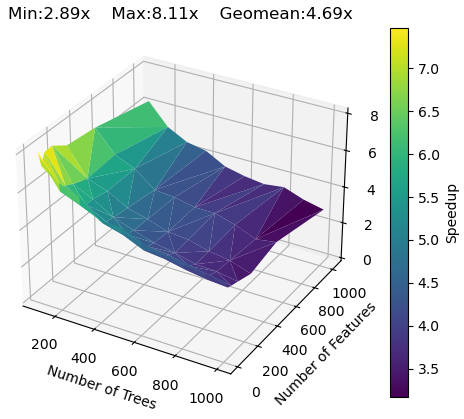
\includegraphics[width=\linewidth]{figures/RandomModels/kernel_speedup_b512_depth8.png}
    %\caption{Batch size 512}
  \end{minipage}
  \begin{minipage}[t]{.475\linewidth}
    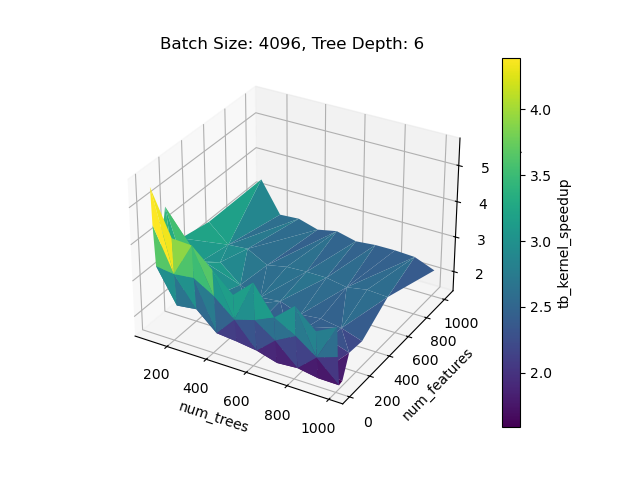
\includegraphics[width=\linewidth]{figures/RandomModels/kernel_speedup_b4096_depth6.png}
    %\caption{Batch size 4096}
  \end{minipage}
  \caption{\label{fig:randomModels4060}\Treebeard{} vs RAPIDs Kernel Time Speedup for random models
  of max depth 8 at batch size 512 and max depth 6 at batch size 4096.}
\end{figure}

% \begin{comment}
\subsubsection*{Synthetic models}
To establish that \Treebeard{} can consistently find betters schedules, we performed an exhaustive comparison between \Treebeard{} and RAPIDS on 700 randomly generated models.   
Figure~\ref{fig:randomModels4060} shows two representative samples of the results, at batch sizes 512 and 4096 on all models, on RTX 4060. 
Each plot shows the speedup of \Treebeard{} over RAPIDS along the z-axis, with the x-axis representing the number of trees and the y-axis the number of features. 
While the exact trends at different batch sizes vary it can be seen that \Treebeard{} consistently outperforms RAPIDS by $1.5-8\times$. Along the tree 
dimension we find that the speedup is very high with fewer trees and stabilizes at around $2\times$ from 300 onwards. We note that \Treebeard{} continues to scale well 
when the number of trees are increased even further. It achieves a speedup of around $2\times$ compared to RAPIDS on \op{letters}, a real-world benchmark
with 26K trees.
%\Treebeard{} consistently outperforms RAPIDS on all models and batch sizes tested.
% \begin{itemize}
%   \item Generated a set of over 700 random models with varying depths (6, 7, 8), number of trees (100 - 1000 in steps of 100), 
%   and number of features (powers of 2 between 8 to 1024 inclusive).
%   \item Compared the kernel time speedup of \Treebeard{} vs RAPIDs on the RTX 4060. The schedule used was the one picked by the auto-tuner. 
%   \item Speedups range between 1.5$\times$ and 8$\times$. \Treebeard{} outperforms RAPIDs on all models and batch sizes tested.
%   \item Figure \ref{fig:randomModels4060} shows the speedup for models of depth 8 and batch size 512 and depth 6 and batch size 4096.
%   Trends for other batch sizes and depths are similar.
% \end{itemize}
\subsubsection*{Utility of Schedule Constructs}
A detailed analysis of the generated schedules indicate that caching, in-memory representation 
and reduction optimizations are crucial for performance. We observe that all three representations 
are necessary, array representation is used 60\% of the time, sparse 30\% of the time and reorg 
10\% of the time for the best schedules on the NVIDIA 4060.  
Shared reduction significantly improves performance especially for multi-class models. For example, 
the \op{letters} and \op{covtype} benchmarks achieves speedups of 1.5$\times$ with shared reduction. 
Shared reduction increases the memory pressure (on shared memory) and not all schedules use it.
While GPUs have a hardware managed cache, explicitly caching the rows using the scheduling primitives 
helps exploit the reuse of rows across trees. We find that caching rows is beneficial for many models
with speedups as large as $1.5\times$ over the best schedule without caching.

\subsubsection*{Comparison on T400}
To test the portability of \Treebeard{}'s techniques, we compare the performance 
of \Treebeard{} on the T400 GPU with RAPIDs and Tahoe. Figure \ref{Fig:TBvsRAPIDsTahoe_T400_Speedup}
shows the speedup of code generated by \Treebeard{} vs RAPIDs and Tahoe on the T400.
Even on the smaller T400 GPU, \Treebeard{} is able to outperform RAPIDs
and Tahoe consistently. We observe similar trends to those on the RTX 4060.

% \subsection{Comparison with RAPIDs, Tahoe and XGBoost}
% \begin{itemize}
%   \item Measured both the kernel time and total time (time including transferring data to the 
%   GPU and results back) for RAPIDs and \Treebeard{}.
%   \item Tahoe only allows us to measure the kernel time since it is written as an executable 
%   that performs inference repeatedly on the same data that is transferred to the GPU once.
%   \item Tahoe does not support multiclass models. We just ran the multiclass models (\op{covtype} and \op{letters})
%   as regression models for the comparison. Tahoe also gives wrong results (as reported by its own tests) for 
%   \op{letters} and \op{year}. In these cases, we pick the time of the fastest variant that gives the correct results.
%   \item Compared the kernel time and total time speedup of \Treebeard{} vs RAPIDs on the RTX 4060 and T400.
%   \item Compared the total time speedup of \Treebeard{} vs XGBoost on the RTX 4060.
%   \item The schedule used was the one picked by the auto-tuner.
%   \item \Treebeard{} outperforms RAPIDs at all batch sizes as shown in Figure \ref{Fig:TBvsRAPIDsTahoe_4060_Speedup}. 
%   \item \Treebeard{} outperforms Tahoe on all models and batch sizes tested. Individual benchmark speedups range between 1.1$\times$ and 16$\times$.
%   \item \Treebeard{} is faster than XGBoost by more than an order of magnitude. Results are not shown because the speedups don't fit on the same graph.
%   \item Figure \ref{Fig:TBvsRAPIDs_4060_TotalTimeSpeedup} shows that \Treebeard{} offers substantial speedup over RAPIDs even when 
%   data needs to be transferred to the GPU and results need to be transferred back.
%   \item Figure \ref{Fig:TBvsRAPIDsTahoe_T400_Speedup} shows that these speedups are also observed on the T400 thus showing 
%   that \Treebeard{} offers portable performance across different GPUs.
%   \item Figure \ref{Fig:KernelTimeIndividualBenchmarks4060} shows that \Treebeard{} outperforms RAPIDs and Tahoe on 
%   individual benchmarks on the RTX 4060 at small (1024) and large (8192) batch sizes. These batch sizes 
%   require different schedules, but the \Treebeard{} auto-tuning heuristic is able to find them.
%   % \item Figure \ref{Fig:TotalTimeIndividualBenchmarks4060} compares the total time of \Treebeard{} vs RAPIDs on individual benchmarks. 
%   % It shows that even with the overhead of data transfers, \Treebeard{} offers significant speedup. The graph in Figure \ref{Fig:TotalTimeIndividualBenchmarks4060} 
%   % shows the breakup of the total time into kernel time and data transfer time.
% \end{itemize}
% \end{comment}

% \begin{figure*}[ht]
%   \centering
%   \begin{subfigure}[b]{.45\textwidth}
%     \subcaptionbox*{}{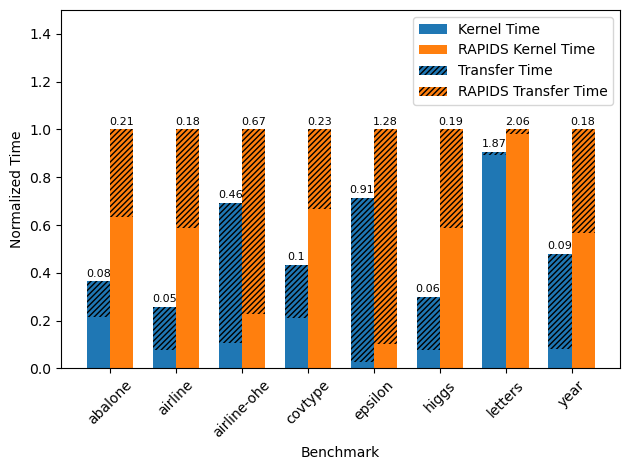
\includegraphics[width=\textwidth]{figures/abs_times_bar_graph_1024.png}}
%     \caption{Batch size 1024.}
%   \end{subfigure}
%   \begin{subfigure}[b]{.45\textwidth}
%     \subcaptionbox*{}{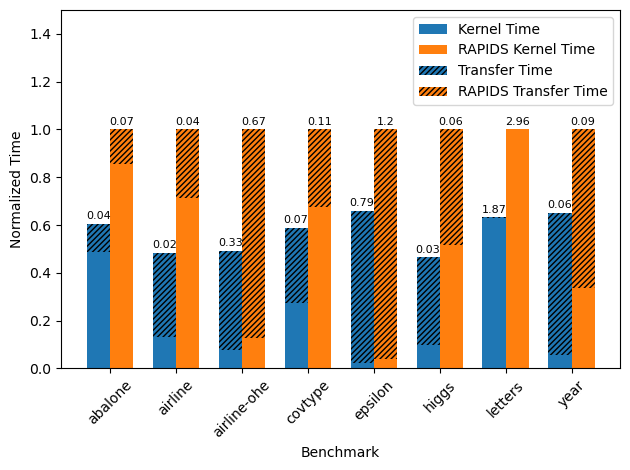
\includegraphics[width=\textwidth]{figures/abs_times_bar_graph_8192.png}}
%     \caption{Batch size 8192.}
%   \end{subfigure}
%   \hfill
%   \caption{\label{Fig:TotalTimeIndividualBenchmarks4060}\Treebeard{} vs RAPIDs total time comparison on NVIDIA RTX 4060. Numbers on the bars are the times 
%   per sample in $\mu$s for \Treebeard{} and RAPIDs. Times for each benchmark are normalized w.r.t the RAPIDs time for that benchmark.}
% \end{figure*}

% \begin{figure}[htb]
%   \centering
%   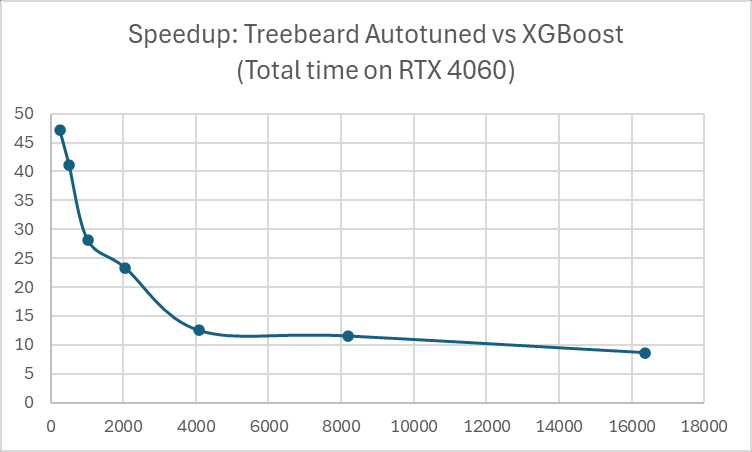
\includegraphics[width=0.75\linewidth]{figures/TBvsXGB_TotalTime.png}
%   \caption{\Treebeard{} vs XGBoost Speedup on RTX 4060.}
%   \label{Fig:TBvsXGBoost_Speedup}
% \end{figure}

\subsection{Performance on AMD GPUs}
While existing systems only support NVIDIA GPUs, we demonstrate that \Treebeard{} 
is able to generate competitive code for AMD GPUs. \Treebeard{} can target AMD GPUs 
because it generates a combination of MLIR's \op{gpu} dialect and LLVM IR 
and these can be JIT'ed to AMD GPUs. While our objective here is not to compare directly 
between AMD and NVIDIA GPUs, we do find that the MI210 achieves better inference times 
on most benchmarks at large batch sizes ($\geq8$k). For example, at a batch size of 16k,
the MI210 is $2\times$ faster than the RTX 4060 on the \op{letters} benchmark. 

\subsection{Schedule Exploration Heuristic}
We evaluated the schedule exploration heuristic described in Section \ref{sec:exploring} on several fronts.
Below we describe the major conclusions we can draw from the evaluation.

\subsubsection*{Efficacy and Speed of Scheduling Heuristic}
Figure \ref{Fig:HeuristicVsFullExplore_Speedup} compares the best schedule found by exhaustive exploration on the RTX 4060 
with the schedule found by the exploration heuristic on RTX 4060.
The plot establishes that the 
heuristic is able to find schedules that are very close to the best schedule (well 
within 5\%) on 4060. The heuristic
is consistently close to two orders of magnitude faster than exhaustive exploration. 
The exploration time ranges between $6$ and $167$ seconds for the heuristic with a mean of $28.7$ seconds.
These results show that our heuristic is able to quickly find schedules that are close to the best schedule.

\subsubsection*{Schedule Sensitivity Across GPUs}
Figure \ref{Fig:AutotuningSpeedupvs4060Sched}
compares the schedule found by the heuristic on T400 and AMD MI210 with the schedule found on the 4060.
It shows that schedule exploration needs to be done on each target to achieve the best performance
and schedules found on one GPU do not always carry over to other GPUs.
For T400, the heuristic is able to find schedules that are 1.05$\times$ to 1.2$\times$ better 
with the maximum difference being $2\times$ (\op{epsilon} at batch size 512).
We find that there is a much larger variation in performance 
between the schedules \Treebeard{} finds on the MI210 compared to the 4060 schedules. For example, 
the geomean speedup over all benchmarks is 1.5$\times$ at batch size 16k and 
The maximum speedup is 2$\times$ for the \op{letters} benchmark at batch size 16k.

% \subsubsection*{Exploration Time}
% Finally, we measure the improvement in exploration time that the heuristic provides 
% compared to exhaustive exploration. Figure \ref{Fig:HeuristicVsFullExplore_Speedup} shows that the heuristic
% is consistently close to two orders of magnitude faster than exhaustive exploration. 
% The exploration time ranges between $6$ and $167$ seconds for the heuristic with a mean of $28.7$ seconds.
% These results show that our heuristic is able to quickly find schedules that are close to the best schedule.

\begin{figure}[htb]
  \centering
  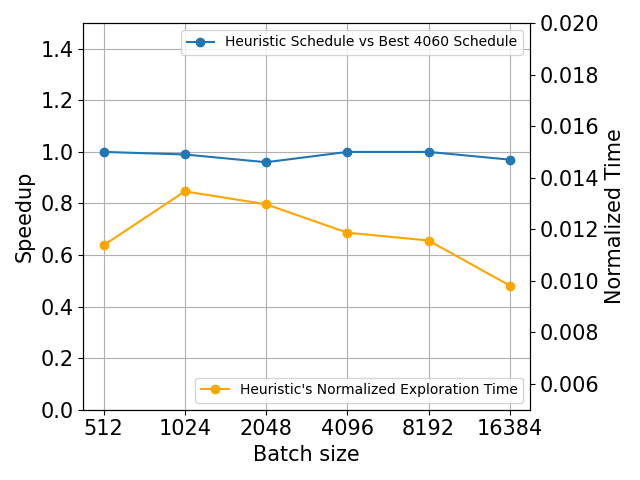
\includegraphics[width=0.75\linewidth]{figures/speedup_vs_norm_time_line_graph_4060.png}
  \caption{Speedup of schedules found by the heuristic vs best schedule found through exhaustive search on NVIDIA RTX 4060 and 
  heuristic schedule exploration time normalized w.r.t full schedule exploration time}
  \label{Fig:HeuristicVsFullExplore_Speedup}
\end{figure}

\begin{figure}[htb]
  \centering
  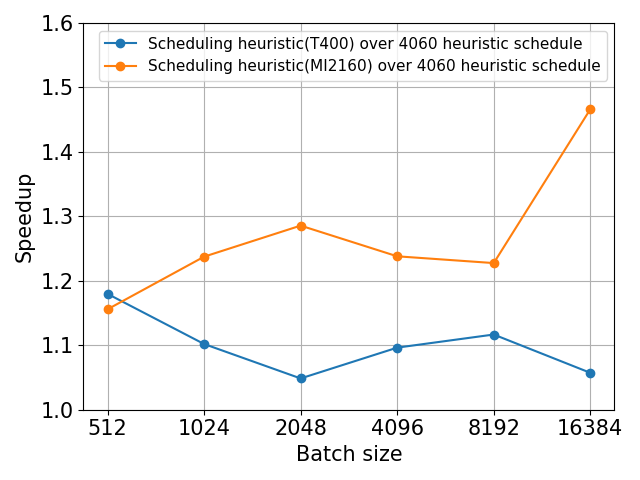
\includegraphics[width=0.75\linewidth]{figures/geomean_speedup_T400_4060_vs_T400_vs_MI2160.png}
  \caption{Geomean speedup of schedule found by exploration heuristic on NVIDIA T400 and AMD MI2160 vs 
  the heuristic schedule on NVIDIA RTX 4060 across batch sizes}
  \label{Fig:AutotuningSpeedupvs4060Sched}
\end{figure}

% \begin{itemize}
%   \item We compare the schedule found by the schedule exploration heuristic on the RTX 4060 with the best schedule found by
%   extensive exploration. Figure \ref{Fig:HeuristicVsFullExplore_Speedup} shows that the heuristic is able to find schedules that are
%   very close to the best schedule found by exhaustive exploration.
%   \item The speedup of the heuristic schedule vs the best 4060 schedule when run on T400 is shown in Figure \ref{Fig:AutotuningSpeedupvs4060Sched}.
%   Geomean speedup ranges from 1.05$\times$ to 1.2$\times$. 
%   \item Unsurprisingly, there is some variation in the best schedule for a model even across NVIDIA GPUs.
% \end{itemize}


% \begin{itemize}
%   \item \Treebeard{} is able to compile code to AMD GPUs. We run generated code on an AMD MI210 GPU.
%   \item None of the other systems we compare against support running on AMD GPUs. This shows the portability of \Treebeard{}.
%   \item The speedup of the heuristic schedule vs the best 4060 schedule when run on the MI210 is shown in Figure \ref{Fig:AutotuningSpeedupvs4060Sched}.
%   \item We see that the geomean speedup over all benchmarks is 1.5$\times$ at batch size 16k.
%   \item The maximum speedup is 2$\times$ for the \op{letters} benchmark at batch size 16k.
% \end{itemize}

\subsection{CPU Improvements}
The enhancements made to the compiler enable \Treebeard{} to explore additional schedules on the CPU
compared to \TreebeardOLD{}. 
In particular, we find that the ability to parallelize across trees improves performance 
significantly at small batch sizes. At batch size 32, we find that the geomean speedup over 
all 8 real-world benchmark models is 2.2$\times$ with a max speedup of 5$\times$. At batch size 64, the average speedup
is 1.1$\times$ with a max speedup of 2$\times$. At batch size 32, parallelizing across trees is faster 
for all models and at batch size 64 the \TreebeardOLD{} schedule that parallelizes across 
rows is faster for only 2 of the 8 models. For small batch sizes, parallelizing across rows does 
not offer the best performance as there is limited reuse of trees in L1 cache.
Also, the amount of work per thread is very small leading to high overheads. 
Parallelizing across trees fixes both these problems. 

\subsection{Discussion}
\subsubsection*{Cost Performance Tradeoff Across Hardware Platforms}
Two of the three GPU targets we use are commodity GPUs that cost less than \$400. They 
are infact much cheaper than the CPU we evaluate on. Despite this, performance on GPUs
is significantly better than on CPUs (by an order of magnitude on RTX 4060).
We believe \Treebeard{} can help enable data scientists to better leverage 
available processors on their systems.

\subsubsection*{A Note on Batch Size}
Batch size is an important parameter dictated by application requirements. It 
exposes a tradeoff between latency and throughput. It is not possible to use 
large batch sizes in latency sensitive applications. Ideally, one would like 
to maximize performance while respecting the batch size constraint imposed 
by the application. \Treebeard{} enables users to explore this tradeoff.  

% \begin{itemize}
%   \item The ability of \Treebeard{} to parallelize across both trees and rows has a significant impact on CPU performance.
%   \item We run experiments on the Intel Core i9-11900K processor to evaluate the impact of parallelizing across trees with small batch sizes. 
%   \item At batch size 32, we find that the average speedup over all 8 models is 2.2$\times$ with a max speedup of 5$\times$.
%   \item At batch size 64, we find that the average speedup over all 8 models is 1.1$\times$ with a max speedup of 2$\times$. 
%   However, we find that 2 of the 8 models show slowdowns in this case. Again, this highlights the need for schedule exploration on CPUs.
%   \item For small batch sizes, parallelizing across rows does not work great since there is limited reuse of trees in L1 cache.
%   Also, the amount of work per thread is very small leading to high overheads. 
%   \item Parallelizing across trees is more effective since there is more reuse in L1 cache and the amount of work per thread is higher.  
% \end{itemize}

Overall, our evaluation shows that \Treebeard{} is able to efficiently generate 
high-performance code for processors ranging from NVIDIA and AMD GPUs to Intel CPUs.
On all platforms and models that we tested on, \Treebeard{} significantly outperforms
state-of-the-art systems like RAPIDs, Tahoe and \TreebeardOLD{}.